\section{Introduction}
Statistical models trained on historical data facilitate several important predictive applications such as fraud detection, recommendation systems, and automatic content classification.
In fact, in one survey, over 60\% of Apache Spark users responded that support for advanced statistical analytics was Spark's most important feature~\cite{sparksurvey}.
This sentiment is echoed across both industry and academia, and there has been significant interest in improving the efficiency of model training workflows~\cite{bdas, alexandrov2014stratosphere, crotty2014tupleware, tensor}. 
An important, yet unfortunately undervalued, step is data pre-processing including structuring data, imputing missing values, and handling incorrect data.
Analysts widely report that this is a significant challenge~\cite{kandel2012,nytimes}, and consequently, it is important to understand if such operations can affect the subsequent statistical models.

While this problem has been well-studied in the context of SQL analytics as \emph{data cleaning}, the effects of cleaning operations can be counter-intuitive in statistical models.
For example, studies have shown that many analysts do not approach cleaning as a one-shot pre-processing step, and instead, repeatedly alternate between cleaning and analysis--using the analysis to guide identification of potential errors~\cite{kandel2012}.
For statistical models, iteratively cleaning some data and re-training leads to biases for even simple models in two dimensions.
Figure \ref{update-arch1}a illustrates training a linear regression on systematically incorrect (shifted) data.
If the analyst only partially cleans the dataset in the first iteration and re-trains the model, the intermediate result can be arbitrarily incorrect with respect to the true model where all of the data are cleaned (Figure \ref{update-arch1}b).
In other words, partial data cleaning may actually make a result worse.
Similarly, high dimensional models face more dramatic sampling effects than the 1D traditional \sumfunc, \countfunc, \avgfunc aggregates (Figure \ref{update-arch1}c).
Data cleaning methodologies designed for SQL analytics, such as Sample-and-Clean~\cite{wang1999sample} and Progressive Data Cleaning~\cite{altowim2014progressive, papenbrock2015progressive, DBLP:journals/pvldb/YakoutENOI11}, will have to be re-thought for the statistical modeling setting, and this paper explores how to apply existing data cleaning algorithms with guarantees of convergence for a large class modeling problems. 

Data cleaning is a broad problem that encompasses extraction, de-duplication, schema matching, and many other problems in relational data.
We focus on two common operations that often necessitate iterative cleaning, removing outliers and attribute transformation.
For example, battery-powered sensors can transmit inaccurate measurements when battery levels are low \cite{DBLP:conf/pervasive/JefferyAFHW06}. 
Similarly, data entered by humans can be susceptible to a variety of inconsistencies (e.g., typos), and unintentional cognitive biases~\cite{DBLP:conf/recsys/KrishnanPFG14}.
Since these two types of errors do not affect the schema or leave any obvious signs of corruption (e.g., NULL values), model training may seemingly succeed--albeit with an inaccurate result.

\begin{figure}[t]
\centering
 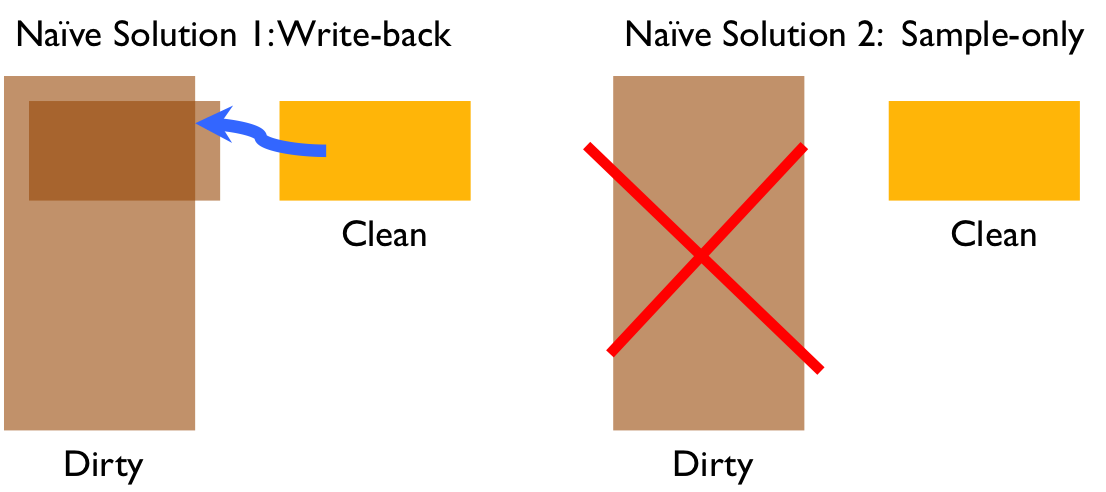
\includegraphics[width=\columnwidth]{figs/update-arch.png}
 \caption{(a) Systematic corruption in one variable can lead to a shifted model. 
 (b) Mixed dirty and clean data results in a less accurate model than no cleaning.
(c) Small samples of only clean data can result in similarly inaccurate models. \label{update-arch1}}
\vspace{-2em}
\end{figure}

We propose \sys, a model training framework that allows for iterative data cleaning while preserving provable convergence properties.
The analyst initializes \sys with a model, a featurization function, and a pointer to a dirty relational table, and the \sys initially returns the model trained on the dirty dataset.
\sys recommends a set of sample data that are possibly dirty based on measuring their impact and prediction accuracy with the current best model.
The analyst can apply value transformations and filtering operations to the sample data, and then prompt the system to iterate. 
\sys will incrementally and safely update the model (as opposed to complete retraining), and present a new sample to clean.
We propose several novel optimizations that leverage information from the model to guide data cleaning towards the records most likely to be dirty and most likely to affect the results.
\sys can also incorporate prior knowledge about records that are likely to be dirty.

From a statistical perspective, our key insight is to model the cleaning-training iteration as a form of Stochastic Gradient Descent, an iterative optimization method.
We treat the dirty model as an initialization, and incrementally take gradient steps towards the global solution (i.e., the clean model).
Our argument ensures global convergence with a provable rate for an important class of models called \emph{convex}-loss models which include SVMs, Linear Regression, and Logistic Regression.
Convexity is a property that ensures that the iterative optimization converges to a true global optimum, and we can apply convergence arguments from convex optimization theory to show that \sys converges.

This paper describes the entire \sys architecture. However, the correctness of many of the components require detailed statistical proofs, which we have included in our extended technical report~\cite{activecleanarxiv}. To summarize our contributions:
\begin{itemize}[noitemsep]
\item \textbf{Correctness} (Section \ref{model-update}). We show how to update a dirty model given newly cleaned data. This update converges monotonically in expectation. For a batch size $b$ and iterations $T$, it converges with rate $O(\frac{1}{\sqrt{bT}})$. 
\item \textbf{Efficiency} (Section \ref{dist-samp}). We derive a theoretical optimal sampling distribution that minimizes the update error and an approximation to estimate the theoretical optimum.
\item \textbf{Detection and Estimation} (Section \ref{opti}). We show how \sys can be integrated with data detection to guide data cleaning towards records expected to be dirty.
\item The experiments evaluate these components on four datasets with real and synthetic corruption (Section \ref{eval}). Results suggest that for a fixed cleaning budget, \sys returns more accurate models than uniform sampling and Active Learning when systematic corruption is sparse.

%For a 5\%  systematic corruption, \sys cleans 55\% fewer records to achieve the same accuracy as an Active Learning algorithm.
\end{itemize}






